\documentclass[11pt]{article}
\usepackage{enumerate}
\usepackage{thmbox}
\usepackage[utf8]{inputenc}
\usepackage{fullpage}
\usepackage{amsmath}
\usepackage{amssymb}
\usepackage{graphicx}
\usepackage{float}
\usepackage{listings}
\usepackage{xcolor}
\usepackage{pdfpages}
\usepackage{caption}
\usepackage{subcaption}
\usepackage{lastpage}
\usepackage[norsk]{babel}

\newenvironment{bottompar}{\par\vspace*{\fill}}{\clearpage}

\DeclareFixedFont{\ttb}{T1}{txtt}{bx}{n}{8} % for bold
\DeclareFixedFont{\ttm}{T1}{txtt}{m}{n}{8}  % for normal

\definecolor{codegreen}{rgb}{0,0.6,0}
\definecolor{codegray}{rgb}{0.5,0.5,0.5}
\definecolor{codepurple}{rgb}{0.58,0,0.82}
\definecolor{backcolour}{rgb}{0.95,0.95,0.92}
 
\lstdefinestyle{mystyle}{
    backgroundcolor=\color{backcolour},   
    commentstyle=\color{codegreen},
    keywordstyle=\color{magenta},
    numberstyle=\tiny\color{codegray},
    stringstyle=\color{codepurple},
    basicstyle=\ttfamily\small,
    breakatwhitespace=false,         
    breaklines=true,                 
    captionpos=b,                    
    keepspaces=true,                 
    numbers=left,                    
    numbersep=3pt,                  
    showspaces=false,                
    showstringspaces=false,
    showtabs=false,                  
    tabsize=3
}
 
\lstset{style=mystyle}

\newcounter{excount}
\newenvironment{exercise}[1][]{\addtocounter{excount}{1} \noindent {\bf Exercise
    \arabic{excount} #1}\hspace{2mm}}{\vspace{4mm}}

\renewcommand{\d}{\mathrm{d}}
%%%%%%%%%%%%%%%%%%%%%%%%%%%%%%%%%%%%%
\newcommand{\ObligNumber}{3 }
%%%%%%%%%%%%%%%%%%%%%%%%%%%%%%%%%%%%%
\begin{document}
\title{\begin{huge}FYS2160 Termodynamikk og statistisk fysikk \end{huge} \\ \begin{Huge}Oblig \ObligNumber\end{Huge}}
\author{Ole Gunnar Johansen}

\maketitle
\noindent
\textit{Denne obligen inneholder \pageref{LastPage} sider. \\ \ \\}
\begin{exercise}
	\begin{itemize}
	
	
	
	
		\item[a)] 
			In a crystal with $N$ atoms and $n$ vacancies, there are in total $N+n$ spots where the atoms can take place. The multiplicity is therefore
			\begin{align}
				\Omega(N,n) = \begin{pmatrix}N+n \\ n \end{pmatrix} = \frac{(N+n)!}{n!N!}
			\end{align}
		
		
		
		
		
		\item[b)]
			The entropy can then be written using the Boltzmann formula:
			\begin{align}
				S 	&= k\ln \Omega \nonumber \\
					&= k \ln \begin{pmatrix}N+n \\ n\end{pmatrix} \nonumber \\
					&= k \ln \left( \frac{(n+N)!}{n!N!} \right) \nonumber \\
					&= k \left[ \ln ((N+n)!) - \ln (n!) - \ln (N!) \right] \label{eq: entropy crystal exact}
			\end{align}
		
		
		
		
		
		\item[c)]
			Using Stirling's approximation:
			\begin{align}
				\ln (x!) \approx \ln \sqrt{2\pi x} + x\ln x - x \approx x\ln x - x,
			\end{align}
			where in the last transition the assumption of large $x$ were made (OK since we are assuming $N>>1$), we can rewrite eq. \eqref{eq: entropy crystal exact}:
			\begin{align}
				S	&\approx k\left[(N+n)\ln (N+n) - (N+n) - n\ln n + n - N\ln N + N \right] \nonumber \\
					&= k\left[(N+n)\ln(N+n) - n\ln n - N \ln N \right] \nonumber \\
					&= k\left[(N+n) \ln \left( N \left( 1+\frac{n}{N} \right) \right) -n \ln n - N \ln N \right] \nonumber \\
					&= k \left[ (N+n) \left( \ln N + \ln \left( 1+\frac{n}{N} \right) \right) - n\ln n - N\ln N \right] \label{eq: entropy crystal simp 1}
			\end{align}
			Using Taylor expansion we get, for small $x$:
			\begin{align*}
				\ln (1+x) = x + O(x^2)
			\end{align*}
			Using this under the assumption $n << N$, we can simplify eq. \eqref{eq: entropy crystal simp 1} to
			\begin{align}
				S 	&\approx kn\left[\ln \left( \frac{N}{n} \right) +\frac{n}{N} + 1  \right] \label{eq: entropy crystal simp final}
			\end{align}
		
		
		
		
		
		\item[d)]
			From the definition of temperature, we have that
			\begin{align}
				\frac{1}{T} = \left( \frac{\partial S}{\partial U} \right) _{N,V} \label{eq: definition temperature}
			\end{align}
			when the number of particles $N$ and the volume $V$ is held constant. To free atoms in the crystal so that there are $n$ vacancies, requires energy equal to
			\begin{align*}
				U = \epsilon_0 + n\Delta \epsilon \Rightarrow n = \frac{U - \epsilon_0}{\Delta \epsilon}
			\end{align*}
			Plugging this back into eq. \eqref{eq: entropy crystal simp final} and using eq. \eqref{eq: definition temperature}, we get
			\begin{align*}
				\frac{1}{T} 	&= \frac{\partial}{\partial U} \left( k \frac{U-\epsilon_0}{\Delta \epsilon} \left( \ln \left( \frac{N \Delta \epsilon}{U-\epsilon_0} \right) + \frac{U-\epsilon_0}{N\Delta \epsilon} + 1 \right)  \right) \\
									&= \frac{k}{\Delta \epsilon} \ln \left( \frac{N\Delta \epsilon}{U-\epsilon_0} \right)  \\
									&= \frac{k}{\Delta \epsilon} \ln \frac{N}{n} \\
			\Rightarrow T	&= \frac{\Delta \epsilon}{k} \left(\ln \frac{N}{n}\right) ^{-1}
			\end{align*}
			
			
			
		
		\item[e)]
			From the previous task, we have
			\begin{align*}
				T = \frac{\Delta \epsilon}{k} \left(\ln \frac{N}{n}\right) ^{-1}
			\end{align*}
			Rearranging, we get
			\begin{align}
				\Rightarrow n = Ne^{-\Delta\epsilon/(kT)} \label{eq: crystal number of vacancies n(T)}
			\end{align}
			
			
			
			
		\item[f)]
			From eq. \eqref{eq: crystal number of vacancies n(T)}, it is evident that in the limit when $T\rightarrow 0$, $n\rightarrow 0$ which was the behaviour we wanted.
		
		
		
		
		\item[g)]
			Assuming $\Delta \epsilon = 1$ eV, the concentration of vacancies $n/N$ is plotted in fig. \ref{fig: concentration of vacancies}
			\begin{figure}[H]
				\centering
				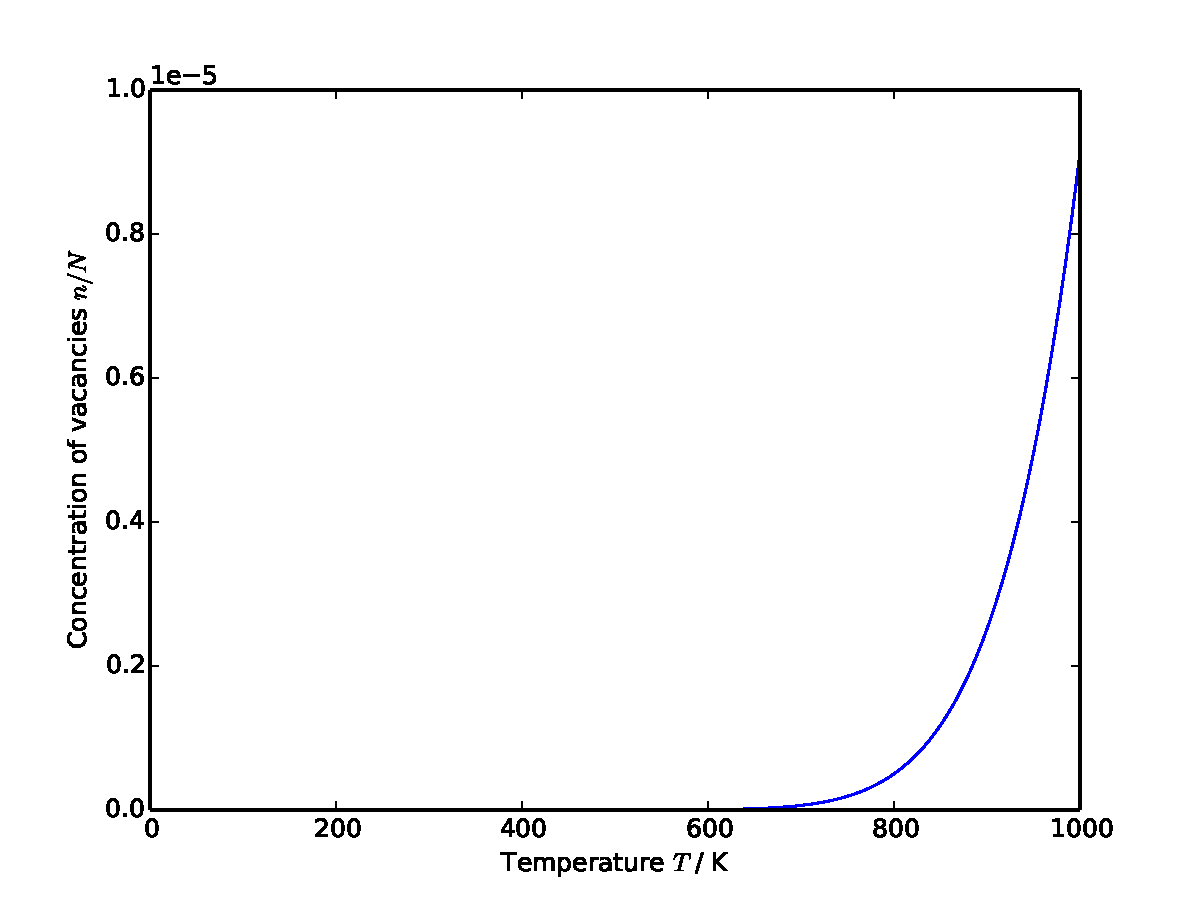
\includegraphics[scale=0.7, clip=true, trim= 0 0 0 0]{FYS2160-oblig-3-fig-conc-n-T.pdf}
				\caption{Concentration of vacancies $n/N$ in the crystal as a function of temperature.}
				\label{fig: concentration of vacancies}
			\end{figure}
		
		
		
		
		\item[h)]
			The heat capacity is defined as
			\begin{align*}
				C_V = \left( \frac{\partial U}{\partial T} \right) _{N,V}
			\end{align*}
			Again, using that the total energy needed to make $n$ vacancies is $U=\epsilon_0+n\Delta \epsilon$. Then $n=(U-\epsilon_0)/\Delta \epsilon$ as above. Eq. \eqref{eq: crystal number of vacancies n(T)} then becomes
			\begin{align*}
				\frac{U-\epsilon_0}{\Delta \epsilon} &= Ne^{-\Delta \epsilon/(kT)} \\
				U &= \Delta \epsilon Ne^{-\Delta \epsilon /(kT)}  + \epsilon_0
			\end{align*}
			so the expression for the specific heat capacity is
			\begin{align*}
				C_V &=  \left( \frac{\partial U}{\partial T} \right) _{N,V} \\
				&= \Delta \epsilon Ne^{-\Delta \epsilon/(kT)} \cdot \frac{\Delta \epsilon}{kT^2} \\
				&= \frac{\Delta \epsilon^2 N}{kT^2}e^{-\Delta \epsilon /(kT)}
			\end{align*}
			Fig. \ref{fig: crystal heat capacity} shows a plot of this in the temperature range from $T=0$ to $T=1000$ K. The heat capacity seems to be very high at high temperatures compared to lower temperatures. Whether or not this is a true behaviour is not easy to say without any experimental data, however, the expression for the heat capacity was derived under the assumption of $n<<N$ - i.e. low temperatures. 1000K may not be a very low temperature.
			\begin{figure}[H]
				\centering
				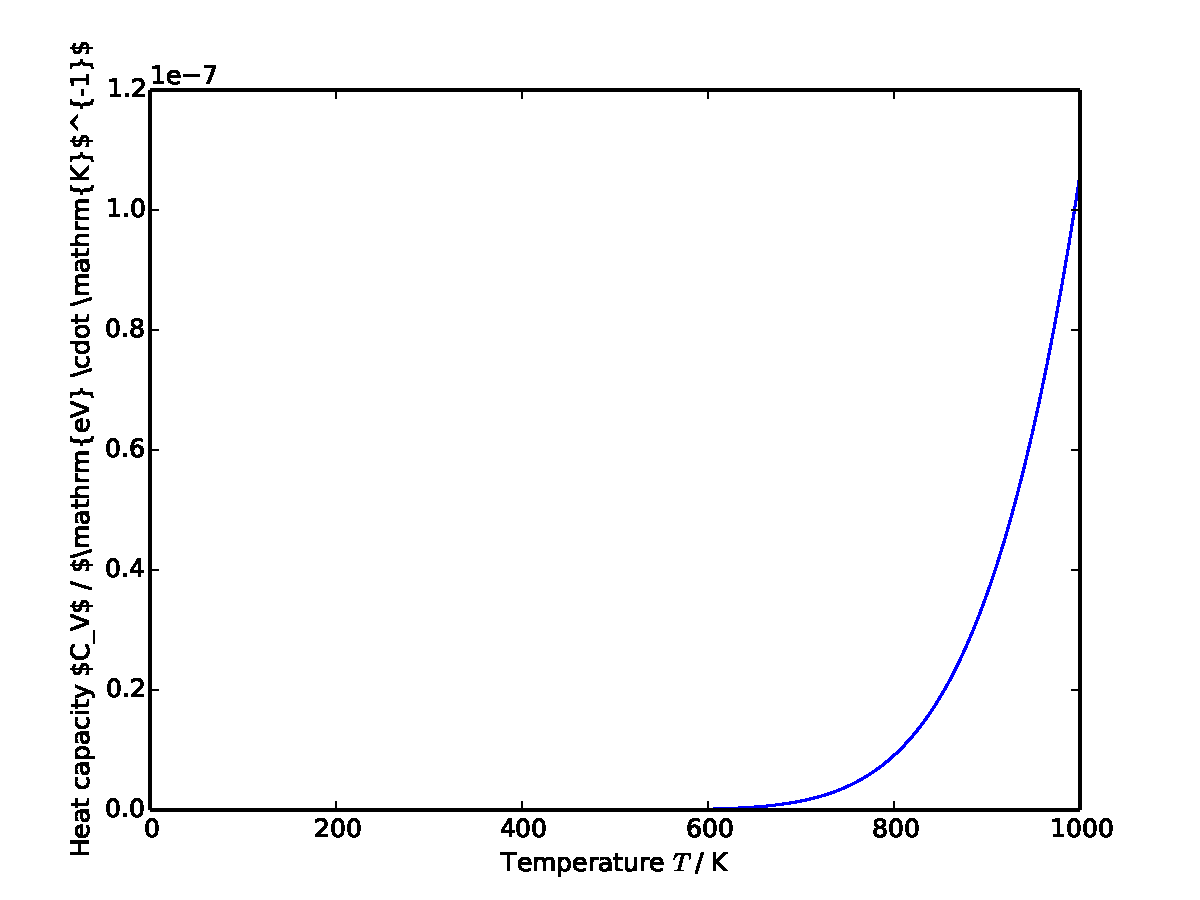
\includegraphics[scale=0.7, clip=true, trim= 0 0 0 0]{FYS2160-oblig-3-fig-heat-capacity.pdf}
				\caption{Specific heat capacity of the crystal as a function of temperature}
				\label{fig: crystal heat capacity}
			\end{figure}
			
			
	\end{itemize}
\end{exercise}



\begin{exercise}
	\begin{itemize}
		\item[a)]
	\end{itemize}
\end{exercise}

\begin{bottompar}
\begin{center}
	Oblig \ObligNumber slutt
\end{center}
\end{bottompar}
\end{document}